\documentclass[answers, a4paper, 11pt]{exam}
\usepackage{amsmath}
\usepackage{amssymb}
\usepackage{amsthm}
\usepackage[italian]{babel}
\usepackage{ccicons}
\usepackage{hyperref} % Has to be loaded before cleveref
\usepackage{cleveref}
\usepackage[utf8]{inputenc} % Has to be loaded before csquotes
\usepackage[autostyle=false, style=english]{csquotes}
\usepackage[margin=2cm]{geometry}
\usepackage{graphicx}
\usepackage{mathrsfs}
\usepackage{multicol}
\usepackage{relsize}

\pagestyle{plain} 
\graphicspath{{./images/}}
\MakeOuterQuote{"}
\setlength{\columnseprule}{.4pt}
\renewcommand{\solutiontitle}{\noindent\textbf{R:}\enspace}
\newcommand{\norm}[1]{\left\lVert#1\right\rVert}
\DeclareMathOperator*{\argmax}{\arg\!\max}
\DeclareMathOperator*{\argmin}{\arg\!\min}
\DeclareMathOperator*{\bigint}{\mathop{\mathlarger{\int}}}
\DeclareMathOperator{\sgn}{sgn}
\DeclareMathOperator{\sca}{sca}
\DeclareMathOperator{\Po}{Po}
\DeclareMathOperator{\Ze}{Ze}
\DeclareMathOperator{\Lapl}{\mathcal{L}}
\def\dbar{{\mathchar'26\mkern-12mu d}}

\title{Controlli Automatici T}
\author{Kevin Michael Frick}
\begin{document}
\maketitle
\section{Domande}
\begin{questions}
\question \textbf{Sistemi dinamici}
\begin{parts}
\part Quali caratteristiche ha un punto di equilibrio?
\begin{solution}Il vettore $\dot{x}$ delle derivate delle variabili di stato è nullo.\end{solution}
\part Come si linearizza un sistema dinamico?
\begin{solution}
Sviluppando in serie di Taylor al primo ordine intorno a un punto di equilibrio 
le espressioni dell'uscita e delle derivate dello stato.\end{solution}
\end{parts}
\question \textbf{Trasformata di Laplace}
\begin{parts}
\part Dimostrare l'espressione della trasformata di Laplace $G(s)$ di un sistema dinamico. 
\begin{solution}
Dall'espressione in forma di stato
\[
\begin{cases}
\dot{x}(t) = A x(t) + B u(t) \\
y(t) = C x(t) + D u(t)
\end{cases}
\]
si ottiene, trasformando secondo Laplace:
\[
\begin{cases}
sX(s) - x_{0} = A X(s) + B U(s)\\ 
Y(s) = C X(s) + D U(s)
\end{cases}
\]
Siamo interessati solo all'evoluzione forzata, quindi $x_{0} = 0$. 
Si ricava l'espressione di $X(s)$:
\[
(sI - A) X(s) = B U(s) \implies X(s) = (sI - A)^{-1} B U(s)
\]
Sostituendo nell'espressione di $Y$ si ha:
\[
Y(s) = (C (sI - A)^{-1} B + D) U(s)
\]
Quindi 
\[
\frac{Y(s)}{U(s)} = C (sI - A)^{-1} B + D = G(s)
\]

\end{solution}
\end{parts}
\question \textbf{Risposte di sistemi elementari}
\begin{parts}
\part Ricavare la risposta allo scalino di un sistema con due poli reali e uno zero. 
Cosa cambia al variare di $T$ e $\tau$? 
\begin{solution}
Un sistema con due poli reali e uno zero (e guadagno unitario) ha trasformata di Laplace 
\begin{equation}
    G(s) = \frac{1 + \tau s}{(1 + T_1 s) (1 + T_2 s)}
\end{equation}
La risposta allo scalino si ricava mediante lo sviluppo in fratti semplici di $\frac{1}{s} G(s)$ ed è pari a \begin{equation}
    y(t) = \sca(t) (1 + \frac{\tau - T_1}{T_1 - T_2} e^{-t/T_1} - \frac{\tau - T_2}{T_1 - T_2} e^{-t/T_1})
\end{equation}
Si distinguono tre casi:
\begin{enumerate}
\item $ \tau > T_1 > T_2 > 0$: il sistema presenta una sovraelongazione tanto più marcata quanto più lo zero è vicino all'origine;
\item $\tau \approx T_1 > T_2$: il sistema è approssimabile con un sistema del primo ordine con un solo polo,
presenta lieve sovraelongazione se $\tau > T_1$ e sottoelongazione se $\tau < T_1$.
\item $\tau < 0, T_1 > T_2$: il sistema presenta una sottoelongazione tanto più marcata quanto più lo zero è vicino all'origine.
\end{enumerate} 
\end{solution}
\part Ricavare la risposta allo scalino di un sistema con una coppia di poli complessi coniugati. 
Cosa cambia al variare di $\xi$?
\begin{solution}
Un sistema con una coppia di poli complessi coniugati e guadagno unitario ha trasformata di Laplace
\begin{equation}
    G(s) = \frac{1}{1 +  2 \xi s / \omega_n + s^2/\omega_n^2}
\end{equation}
La risposta allo scalino si ricava mediante lo sviluppo in fratti semplici di $\frac{1}{s}G(s)$ e, per $\xi \in ]0, 1[$, è pari a
\begin{equation}
    y(t) = \sca(t) (1 - \frac{e^{-\xi\omega_n t}}{\sqrt{1-\xi^2}}\sin(\omega_n\sqrt{1-\xi^2}t + \arccos(\xi)))
\end{equation}
Si dimostra che $S_\% = 100e^\frac{-\pi\xi}{\sqrt{1-\xi^2}}$. 
È possibile approssimare il tempo di assestamento al $k\%$ con l'istante di tempo in cui $e^{\-\xi\omega_n t} = k/100$.
Si ottiene quindi $T_{ak} \approx \bar{t}_k = -\frac{\log(k /100)}{\xi\omega_n}$.
Se $\xi = 0$ il sistema è stabile, non asintoticamente, mentre per $\xi < 0$ il sistema diventa instabile.
\end{solution}
\end{parts}
\question \textbf{Risposta in frequenza}
\begin{parts}
\part Regole per il tracciamento approssimato dei diagrammi di Bode. 
\begin{solution}
Prendendo i logaritmi dei moduli, i prodotti e i quozienti diventano somme e differenze: 
è quindi possibile separare i contributi di guadagno $k$, zeri/poli reali e cc e poi sommarli per ottenere il diagramma di Bode finale.
I contributi degli zeri si ottengono negando quelli dei poli.
Lo stesso vale per gli argomenti.

\textbf{Modulo}

\begin{enumerate}
\item Guadagno $k$: Retta orizzontale che vale $20 \log_{10} k$;
\item Poli nell'origine $(j\omega)^g$: Retta con pendenza $-20g$ dB/decade;
\item Poli reali $1 + \tau j\omega$: Retta con pendenza -20 dB/decade per $\omega > 1 / |T|$;
\item Poli cc $1 + 2 j \omega \xi / \omega_n - \omega^2 / \omega_n^2$: Retta con pendenza -40 dB/decade per $\omega > \omega_n$.
\end{enumerate}

\textbf{Argomento}

\begin{enumerate}
\item Guadagno $k$: 0 per guadagno positivo, $-180^\circ$ per guadagno negativo;
\item Poli nell'origine $(j\omega)^g$: $-g 90^\circ$ su tutto l'asse delle pulsazioni;
\item Poli reali $1 + \tau j \omega$: $-90^\circ \sgn(T)$ per $\omega > \frac{1}{|\tau|}$;
\item Poli cc $1 + 2 j \omega \xi / \omega_n - \omega^2 / \omega_n^2$: $-180^\circ \sgn(\xi)$ per $\omega > \omega_n$.
\end{enumerate}

\end{solution}
\end{parts}
\question \textbf{Stabilità e prestazioni}
\begin{parts}
\part Definizione di margine di ampiezza e fase. In che modo questi margini danno indicazioni sulla stabilità robusta del sistema?
\begin{solution}
Il margine di fase è definito come $M_f = 180^\circ + \arg\{L(j\omega_c)\}, |L(j\omega_c)|_{dB} = 0$, quello di ampiezza come $M_a = -|L(j\omega_\pi)|, \arg\{L(j\omega_\pi)\} = -180^\circ$. 
Il margine di fase dà una misura della stabilità del sistema a fronte di un ritardo di tempo: dato che un ritardo di tempo $\tau$ dà al diagramma di Bode della fase un contributo di $-\omega\tau$ il sistema rimane stabile finché $\tau < \frac{M_f}{\omega_c}$.
Lo stesso vale per il margine di ampiezza e incertezze sul guadagno del sistema, che rimane stabile finché l'incertezza $\delta k < M_a$.
\end{solution}
\part Regole per il tracciamento approssimato del luogo delle radici.
\begin{solution}
\begin{enumerate}
\item Il luogo delle radici ha $p$ rami;
\item il luogo delle radici è simmetrico rispetto all'asse reale;
\item tutti i punti dell'asse reale a sinistra di un numero dispari di singolarità reali appartengono al luogo delle radici;
\item i rami partono dai poli di $L(s)$;
\item $z$ rami arrivano agli zeri di $L(s)$, i restanti $p - z$ divergono all'infinito;
\item i rami che divergono hanno asintoti obliqui che intersecano l'asse reale in $x_a = \frac{1}{p - z} \sum (z_i - p_i)$ con $z_i \in \Ze\{L(s)\}, p_i \in \Po \{L(s)\}$ e formano con esso angoli pari a $\frac{(2k + 1) 180^\circ}{p - z}, k \in [1..(p - z)]$;
\item i punti di intersezione dei rami con l'asse reale sono dati dai massimi e minimi di $\gamma(s) = - (1 / L(s))$: i massimi di $\gamma$ rappresentano rami che si separano e diventano cc, i minimi rami che confluiscono sull'asse reale.
\end{enumerate}
\end{solution}
\part Derivare le espressioni delle funzioni di sensitività $F(s), S(s), Q(s)$ e le espressioni approssimate dei loro moduli.
\begin{solution}
A partire dal modello nella prima figura, sfruttando il principio di sovrapposizione
degli effetti si definiscono le uscite $Y_w (s), Y_d (s), Y_n (s)$ dovute 
rispettivamente al riferimento, al disturbo sull'uscita e al disturbo di misura.
In maniera analoga si definiscono gli errori e le variabili di controllo $E_{w, d, n} (s), U_{w, d, n} (s)$.
A questo punto, analizzando un'uscita per volta, è possibile scomporre il modello 
nella somma dei tre modelli rappresentati nelle figure successive.

{
	\centering

	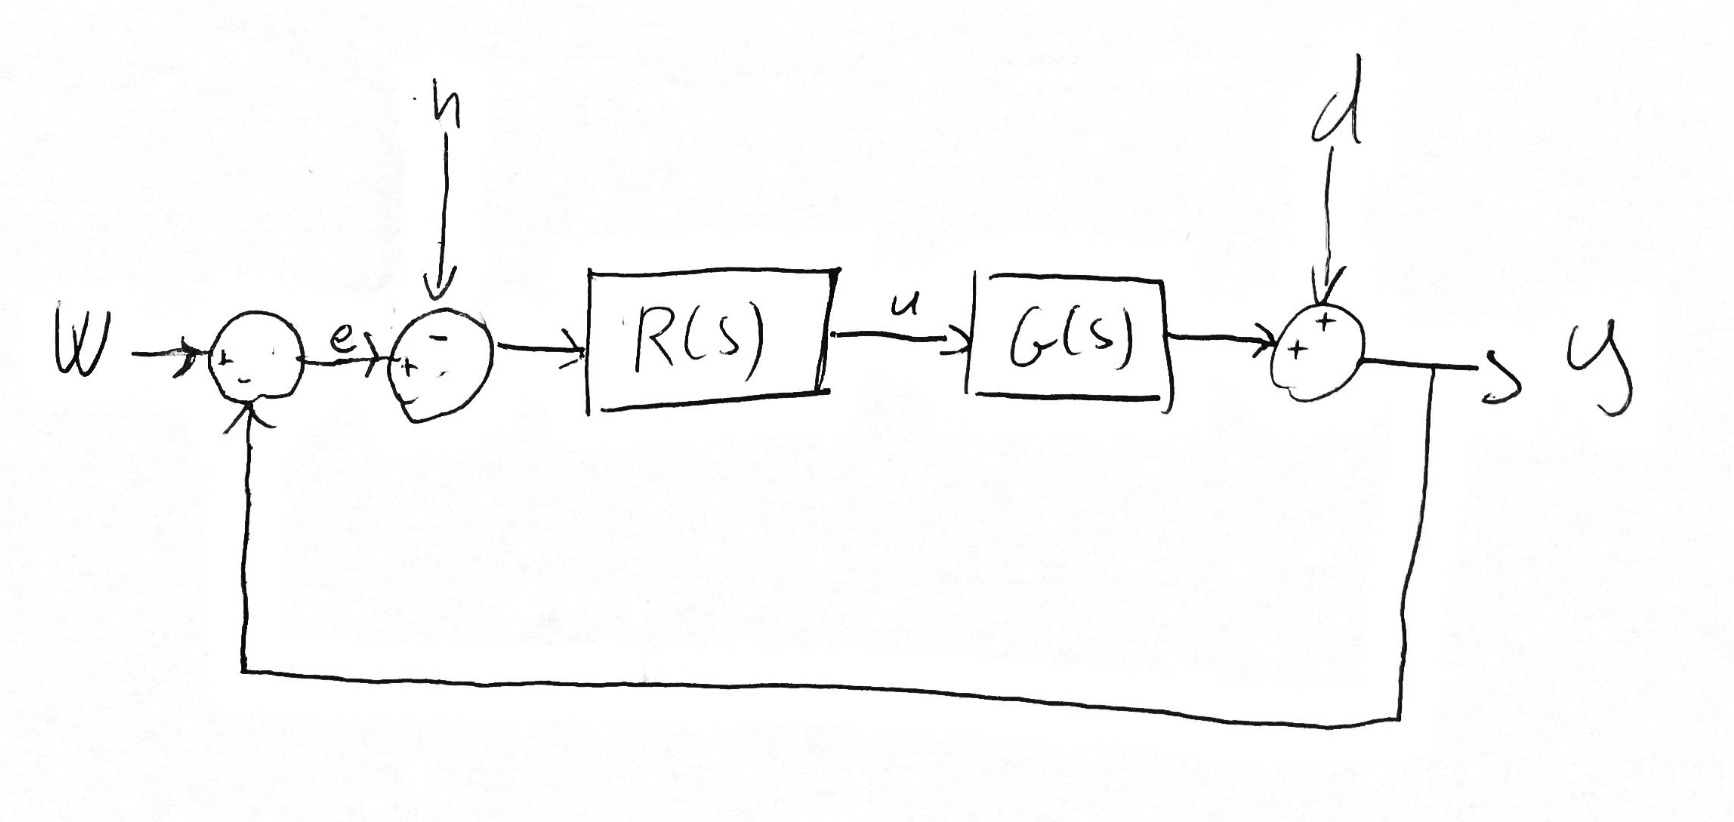
\includegraphics[width=0.75\textwidth]{Model}

}

Analizzando l'uscita dovuto al riferimento, si ha $(W(s) - Y_w(s)) L(s) = Y_w (s) 
\implies Y_w(s) (1 + L(s)) = W(s) L(s) 
\implies \frac{Y_w(s)}{W(s)} = \frac{L(s)}{1 + L(s)} = F(s)$ (prima figura).

Analizzando l'errore dovuto al riferimento, si ha $E_w(s) L(s) = E_w (s) + W(s) 
\implies \frac{E_w(s)}{W(s)} = \frac{1}{1 + L(s)} = S(s)$ (seconda figura).

Analizzando la variabile di controllo dovuta al riferimento, si ha $(W(s) - U_w(s)) R(s) = U_w(s) 
\implies U_w(s) = W(s) \frac{R(s)}{1 + R(s) G(s)} 
\implies \frac{U_w (s)}{W(s)} = \frac{R(s)}{1 + R(s) G(s)} = Q(s)$ (terza figura).

{

\centering
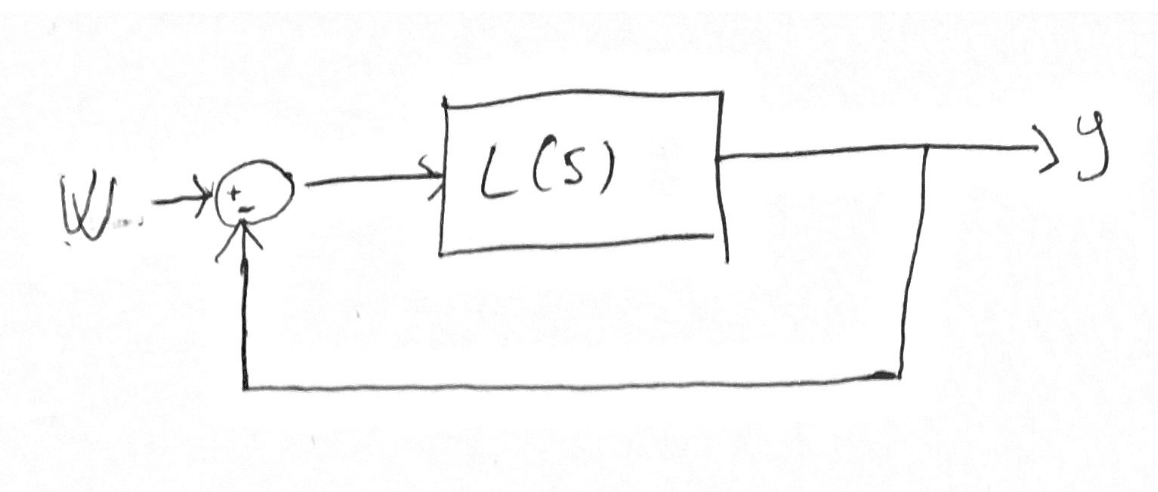
\includegraphics[width=0.3\textwidth]{F}
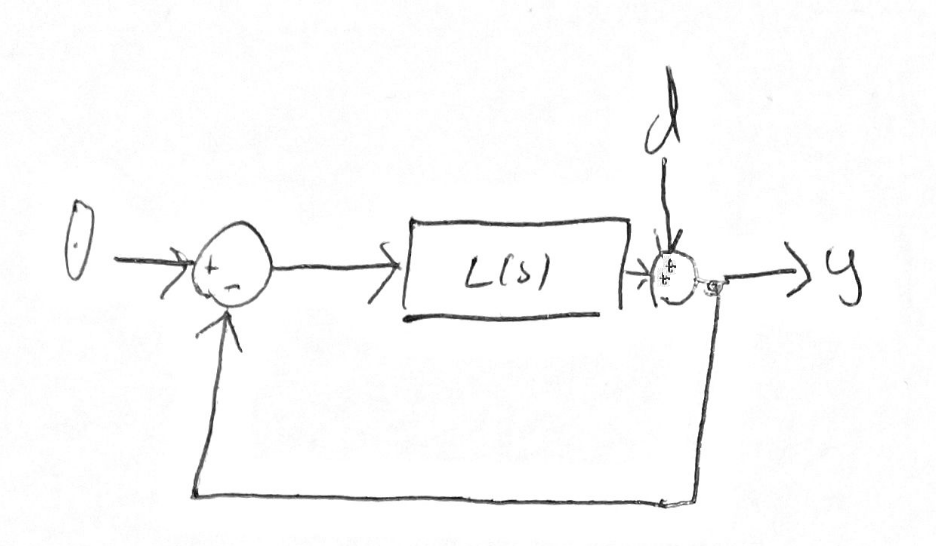
\includegraphics[width=0.3\textwidth]{S}
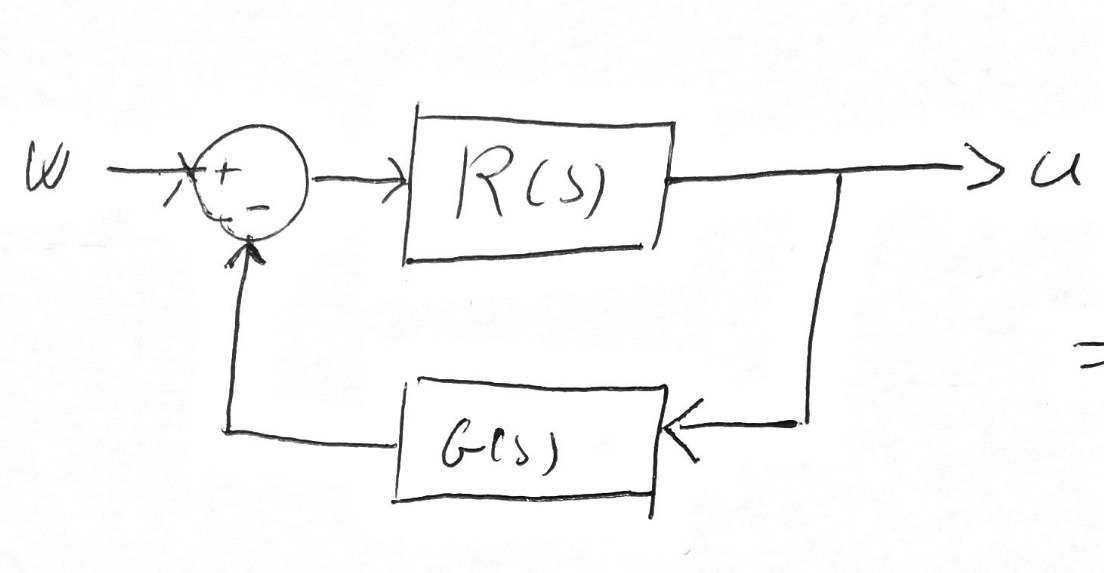
\includegraphics[width=0.3\textwidth]{Q}

}

Per valori alti di $|L(j\omega)|$ (e quindi $\omega < \omega_c$) si ha $|1 + L(j\omega)| = |L(j\omega) + o(L(j\omega))|$, per valori bassi di $L(j\omega)$ invece $|1 + L(j\omega)| = |1 + o(1)|$ , quindi 
\begin{equation}
    |F(j\omega)| \approx 
    \begin{cases}
1 & \omega < \omega_c \\ |L(j\omega)| & \omega > \omega_c
\end{cases}
\end{equation}

\begin{equation}
|S(j\omega)| \approx 
\begin{cases}\frac{1}{|L(j\omega)|} = -|L(j\omega)|_{dB} & \omega < \omega_c \\
1 & \omega > \omega_c
\end{cases}
\end{equation}

\begin{equation}
    |Q(j\omega)| \approx \begin{cases}
    \frac{|R(j\omega)|}{|R(j\omega)G(j\omega)|} = \frac{1}{|G(j\omega)|} & \omega < \omega_c \\
    \frac{|R(j\omega)|}{1} = |R(j\omega)| & \omega > \omega_c
    \end{cases}
\end{equation}

\end{solution}
\part Criterio di Bode. 
\begin{solution}
Un sistema dinamico $L(s)$ con più poli che zeri è asintoticamente stabile se e solo se:
\begin{enumerate}
\item $L(s)$ non ha poli a parte reale strettamente positiva;
\item il diagramma di Bode di $|L(s)|$ interseca una sola volta l'asse delle pulsazioni;
\item $k_s > 0$;
\item $M_f > 0$.
\end{enumerate}
\end{solution}
\end{parts}
\question \textbf{Progetto di regolatori}
\begin{parts}
\part Tracciare un diagramma di flusso con le fasi del progetto di un regolatore.
\begin{solution}

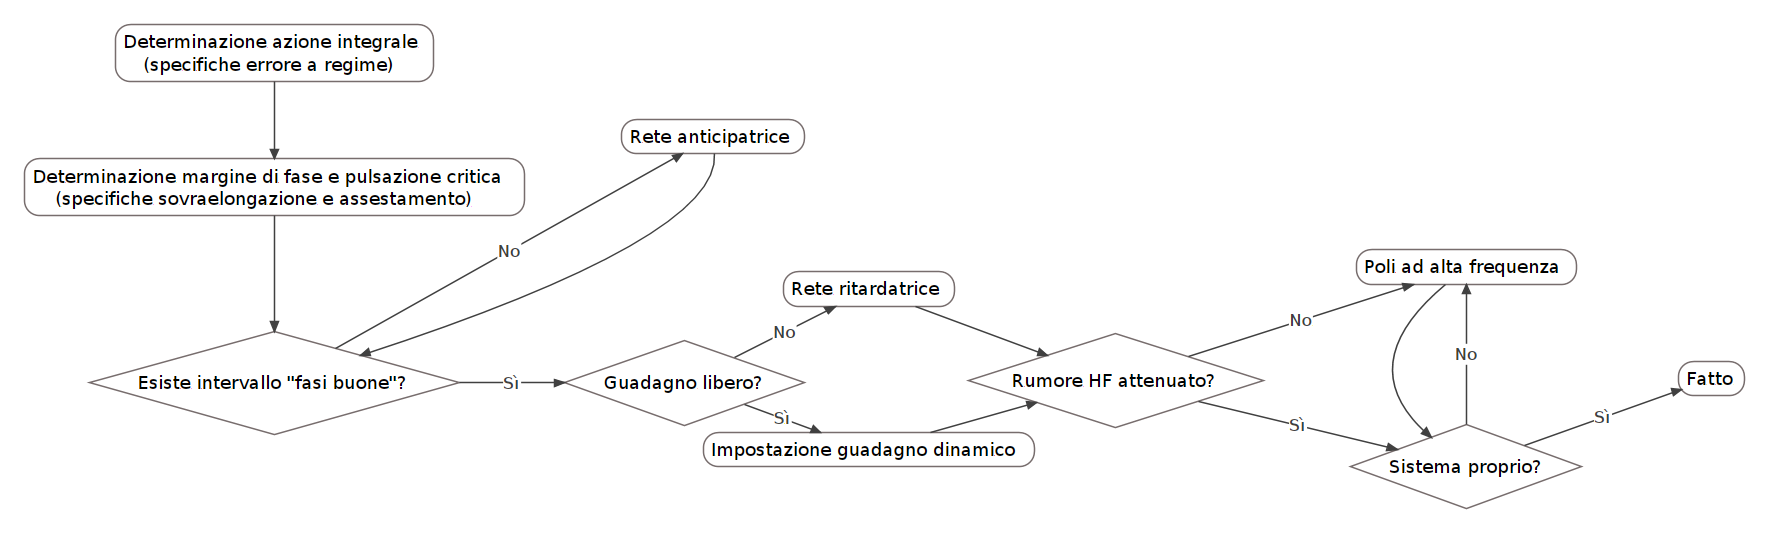
\includegraphics[width=\textwidth]{ProgettoRegolatore}

\end{solution}
\part Perché può essere utile cancellare un polo nell'origine inserendo uno zero nel regolatore dinamico?
\begin{solution}
Perché un solo polo nell'origine è sufficiente per garantire errore a regime nullo;
ogni polo in più toglie 90 gradi alla fase del sistema, abbassando il margine di fase.

Un solo polo nell'origine permette di avere errore a regime nullo per un ingresso a scalino: se $W(s) = \Lapl\{W\sca(t)\} = \frac{W}{s}$ allora, per il teorema del valore finale, $$e_\infty = \lim_{t \rightarrow \infty} e(t) = \lim_{s\rightarrow 0} s E(s) = \lim_{s\rightarrow 0} S(s) W(s) = W \lim_{s \rightarrow 0} S(s) =$$ $$= W \lim_{s \rightarrow 0} \frac{1}{1 + N(s) / s^g D^*(s)} = W \lim_{s \rightarrow 0} \frac{s^g D^*(s)}{s^g D^*(s) + N(s)}$$
Dato che $\lim_{s \rightarrow 0} N(s) = k$ e $\lim_{s \rightarrow 0} D^*(s) = 1$ si ha $$e_\infty = \lim_{s \rightarrow 0} \frac{W s^g}{k + s^g} = \begin{cases}
\frac{W}{1 + k} & g = 0 \\
0 & g > 0
\end{cases}$$

Il risultato si può generalizzare a ingressi a rampa, parabola, ecc. (con trasformata $W/s^p$) ottenendo $$e_\infty = \lim_{s \rightarrow 0} \frac{W s^{g - p + 1}}{k + s^{g}} = \begin{cases}
\frac{W}{k} & g = p - 1 \\
0 & g > p - 1 \\
\infty & g < p - 1
\end{cases}$$
\end{solution}
\part In quali scenari ci si può trovare durante la sintesi di un regolatore?
\begin{solution}
\begin{enumerate}
\item Se c'è un intervallo di pulsazioni tali che, se la pulsazione critica ricade
in quell'intervallo, il margine di fase è pari o superiore a quello desiderato, 
allora è necessario attenuare il diagramma delle ampiezze alterando il meno possibile la fase: 
\begin{enumerate}
\item se si ha guadagno dinamico libero, scegliere $k_d = 10^{-\frac{1}{20} |G_e(j \bar{\omega}_c)|_{dB}}$;
\item altrimenti si attenua mediante l'inserimento di poli e zeri, definendo una 
\textit{rete ritardatrice} nella forma $R_d(s) = \frac{1 + a T s}{1 + T s}, 
0 < a < 1 (\implies aT < T)$ che attenua l'ampiezza per $\omega > 1 / T$ e il cui 
contributo di fase è quasi nullo per le stesse pulsazioni;
\end{enumerate}
\item se non c'è un intervallo di "fasi buone", invece, è necessario alzare 
il diagramma delle fasi alterando il meno possibile l'ampiezza per ricondursi 
allo scenario precedente: si definisce quindi una \textit{rete anticipatrice}
nella forma $R_d(s) = \frac{1 + T s}{1 + a T s}, 0 < a < 1 (\implies a T < T)$,
che aumenta la fase di circa 90 gradi nell'intervallo $[\frac{1}{T}, \frac{1}{aT}]$, 
aumentando però progressivamente anche l'ampiezza per $\omega > \frac{1}{T}$.
\end{enumerate}
\end{solution}
\part Quale valore deve assumere, la $F(s)$ per abbattere 
di $K$ dB un rumore ad alta frequenza? Come si mappa questo requisito sulla $L(s)$? Quale valore deve invece assumere la $S(s)$ e quindi la $L(s)$ per abbattere di $K$ dB un rumore a bassa frequenza? Come si traducono le approssimazioni di $|Q(s)|$ sul progetto di un regolatore?
\begin{solution}Il requisito sull'abbattimento del disturbo di misura in alta frequenza impone che $|F(s)|_{dB} \le -K [dB]$.
Si ha che $\omega > \omega_c \implies |F(s)| = \frac{|L(s)|}{|1 + L(s)|} \approx |L(s)| \implies |L(s)|_{dB} \le -K [dB]$.

Per abbattere invece un disturbo in bassa frequenza è necessario che $|S(s)|_{dB} \le K [dB]$, quindi dato che $ |L(j\omega)|_{dB} \approx -|S(j\omega)|_{dB} (\omega < \omega_c) $ si richiede che $|L(j\omega)|_{dB} \ge -K [dB] $.

Infine, dato che $|Q(j\omega)| \approx \frac{1}{|G(j\omega)|} (\omega < \omega_c)$, non è possibile influenzare la variabile di controllo con il regolatore a basse frequenze: è quindi importante non avere valori di $\omega_c$ troppo alti.
\end{solution}
\part Come si ricavano i vincoli sul margine di fase ($M_f \omega_c 
\approx \frac{460}{T^*}$) e sui poli complessi coniugati ($\xi 
\approx \frac{M_f}{100}$) a partire da specifiche sulla sovraelongazione e 
sul tempo di assestamento e quali approssimazioni sono necessarie?
\begin{solution}
La seguente discussione è valida se la funzione $F(s)$ ha una coppia di poli cc dominanti con $\omega_n \approx \omega_c$.
Lo studio della risposta allo scalino di un sistema del secondo ordine con poli cc
permette di affermare che $S_\% = 100 e^\frac{-\pi\xi}{\sqrt{1-\xi^2}}$ e 
$T_{a1} \approx \frac{4.6}{\xi\omega_n}$.
Per $s = j\omega_c$ si ha che \[\frac{|L(s)|}{|1 + L(s)|} = \frac{1}{|1 + e^{j(\pi-M_f^{(rad)})}|} 
= \frac{1}{\sqrt{(1 + \cos(\pi - M_f^{(rad)}))^2+ \sin^2(\pi - M_f^{(rad)})}}\]
\[
= \frac{1}{\sqrt{2 - 2\cos(M_f^{(rad)})}} 
= \frac{1}{2 \sin(M_f^{(rad)}/2)}\]
Ma $F(j\omega_c) = \frac{1}{2\xi}$, quindi \[\frac{1}{2\xi} = \frac{1}{2\sin(M_f^{(rad)}/2)} 
\implies \xi \approx M_f^{(rad)}/2 = \frac{M_f}{2} \frac{\pi}{180} 
\implies \xi \approx \frac{M_f}{100}\]
da cui
\begin{equation}
    T_{a1} \approx 100 \frac{4.6}{M_f \omega_n} \implies M_f \omega_n \approx M_f \omega_c \approx \frac{460}{T_{a1}}
\end{equation}
\end{solution}
\part Come si mappa una specifica sul tempo di assestamento nel luogo delle radici?
\begin{solution}
Tramite un vincolo sulla parte reale dei poli in anello chiuso: $\sigma \le -\log(0.01k)/T_{ak}^*$. 
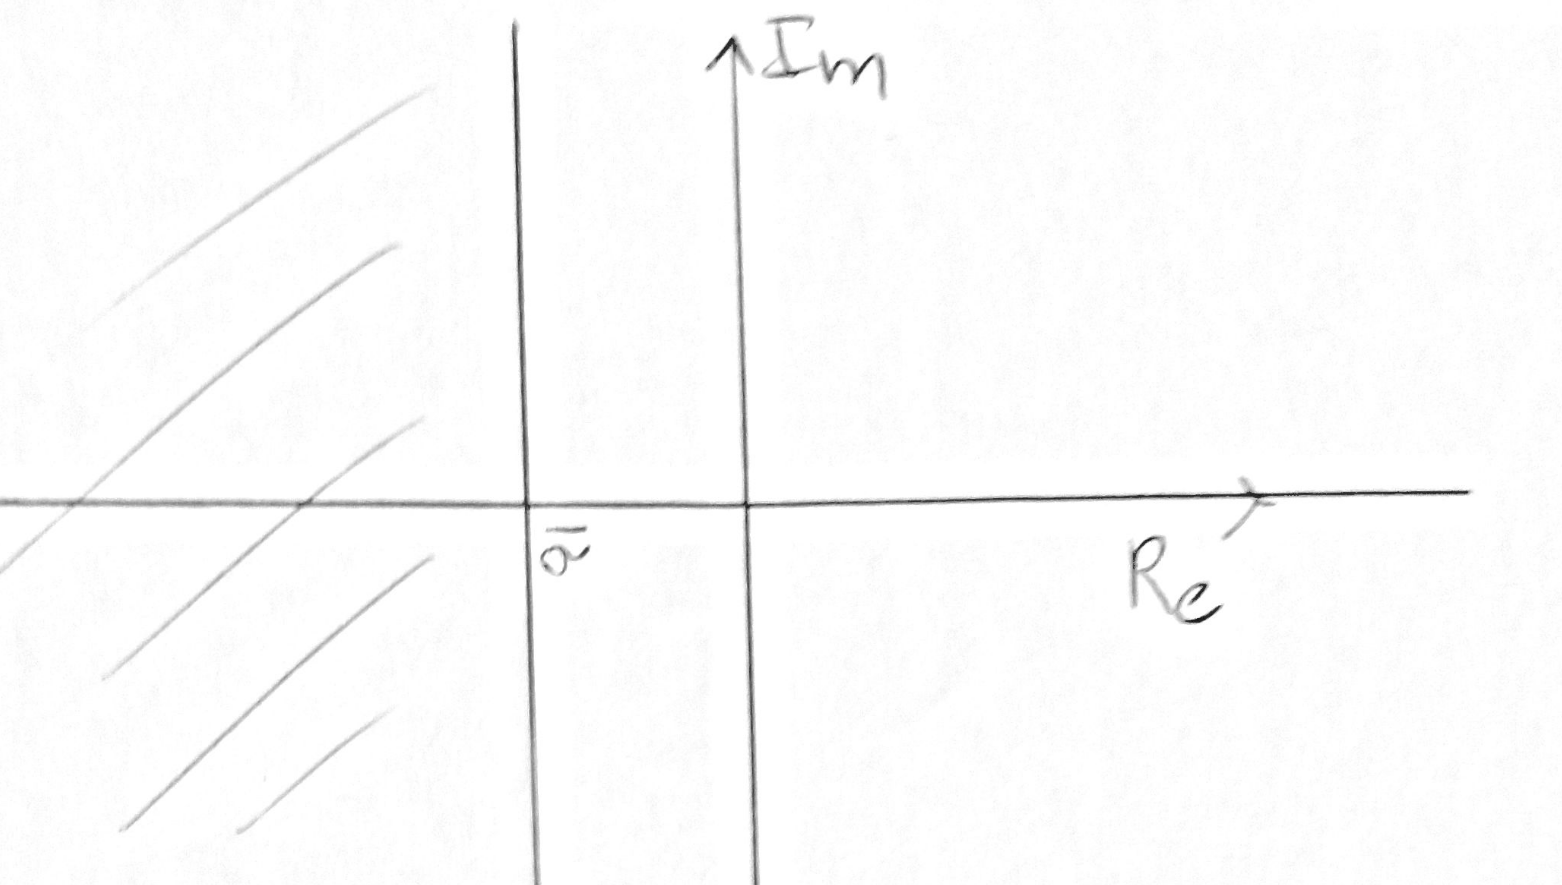
\includegraphics[width=0.5\textwidth]{RLTime}
\end{solution}
\part Come si mappa una specifica sullo smorzamento dei poli dominanti nel luogo delle radici?
\begin{solution}
Perché i poli dominanti abbiano uno smorzamento maggiore di una soglia $\bar{\xi}$, i poli in anello chiuso devono essere all'interno del settore circolare che forma con l'asse reale un angolo pari a $180^\circ - \arccos{\bar{\xi}}$.

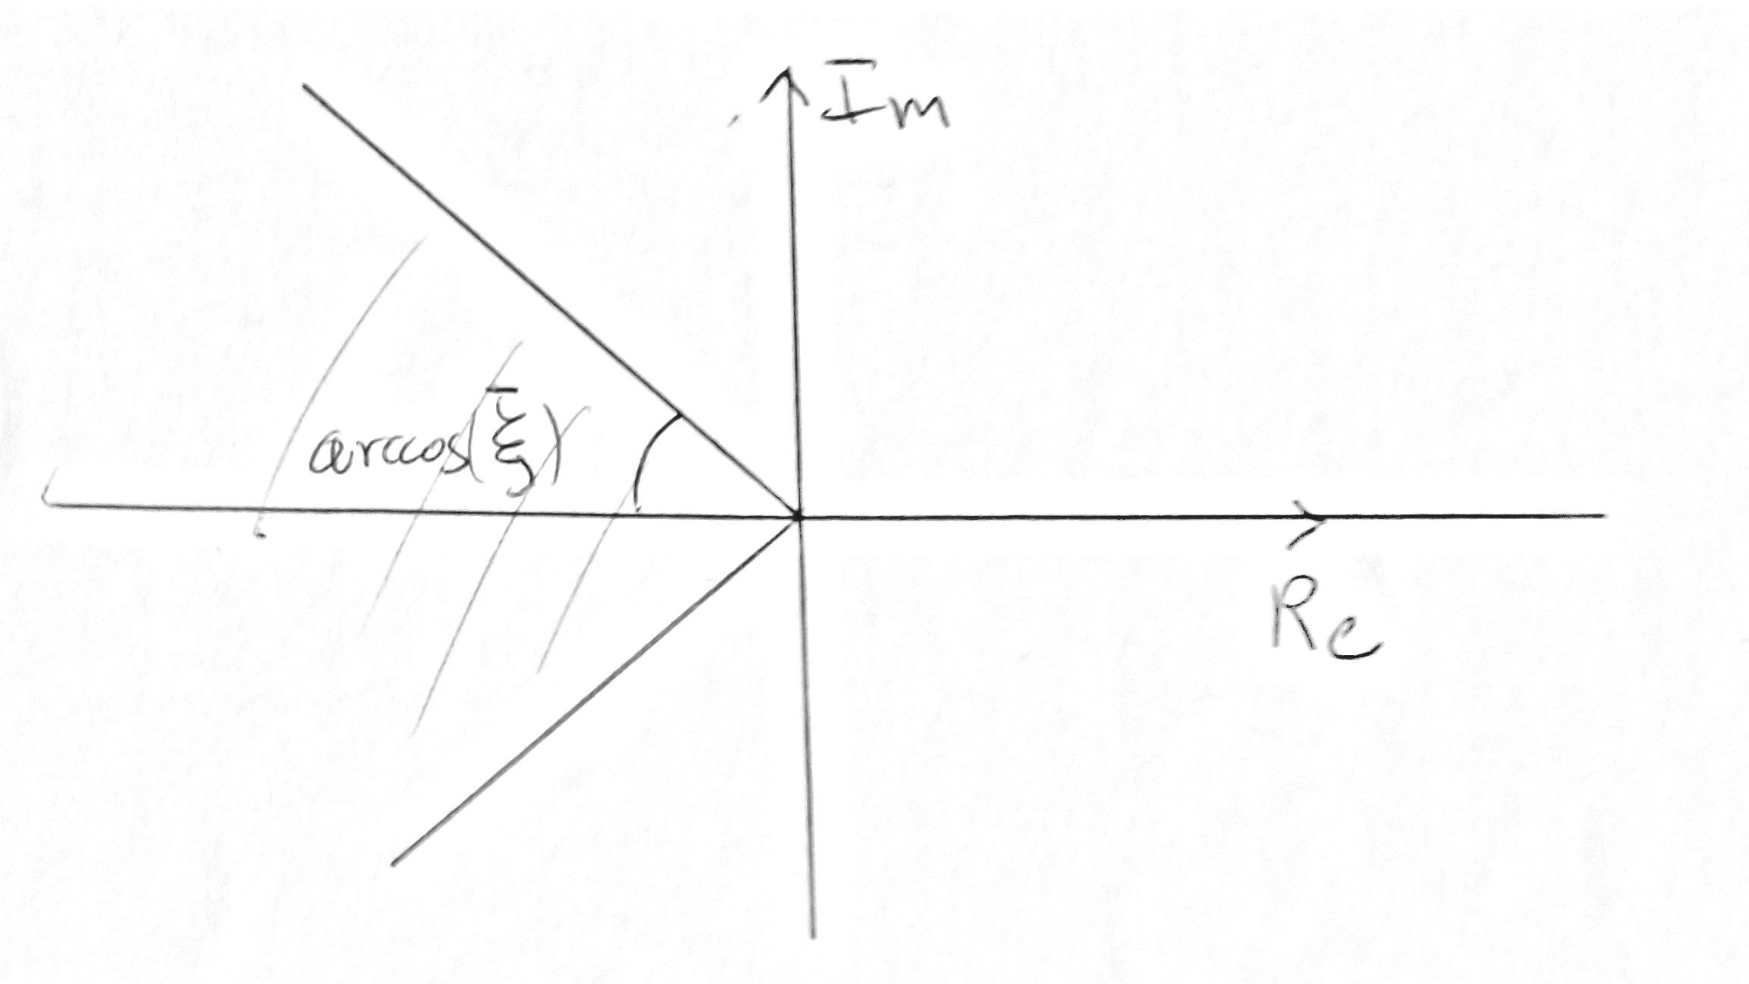
\includegraphics[width=0.5\textwidth]{RLDamp}

\end{solution}
\part Come si mappa una specifica sulla pulsazione naturale dei poli dominanti nel luogo delle radici?
\begin{solution}
Perché la pulsazione naturale dei poli dominanti sia maggiore di una soglia $\bar{\omega}_n$, i poli in anello chiuso devono essere all'esterno della circonferenza con centro nell'origine e raggio $\bar{\omega}_n$.

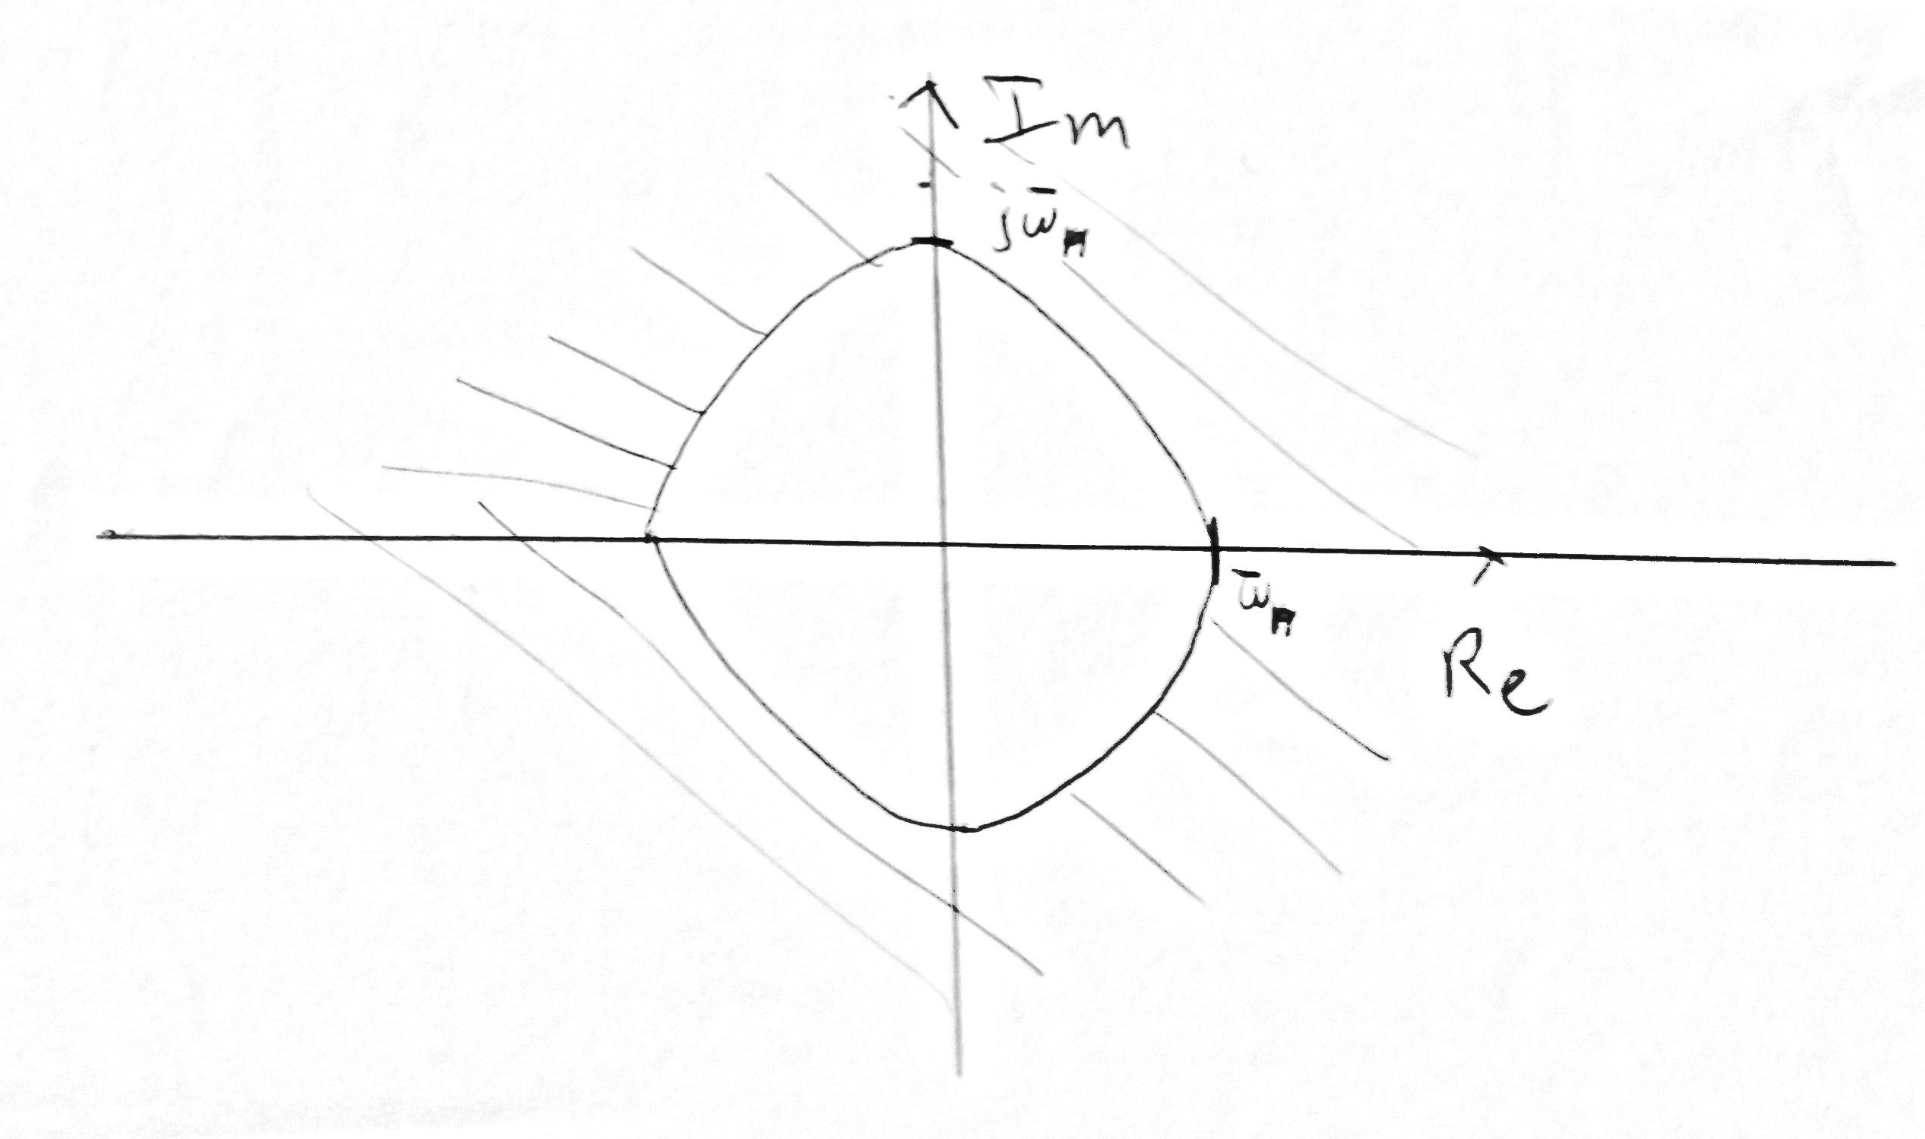
\includegraphics[width=0.5\textwidth]{RLFreq}


\end{solution}\end{parts}
\end{questions}
\ifprintanswers
\pagebreak
\section{Formulario}
\begin{multicols}{2}
Sistemi con uno zero:
\begin{equation}
y(t) =\sca(t)(1 - e^{-t/T})
\end{equation}
Sistemi con uno zero e due poli:
\begin{equation}
y(t) = \sca(t)(1 + \frac{\tau - T_1}{T_1 - T_2} e^{-t/T_1} - \frac{\tau - T_2}{T_1 - T_2} e^{-t/T_2})
\end{equation}
Sistemi con una coppia di poli cc:
\begin{equation}
y(t) = \sca(t)(1 -  \frac{e^{-\xi \omega_n t}}{\sqrt{1 - \xi^2}}  \sin(\omega_n\sqrt{1 - \xi^2} t + \arccos(\xi)))
\end{equation}

\begin{equation}
S_\% = 100e^\frac{-\pi\xi}{\sqrt{1 - \xi^2}}
\end{equation}

\begin{equation}
 T_{ak} \approx \bar{t}_{k} = -\frac{\log(0.01 k)}{\xi \omega_n}
\end{equation}

\begin{equation}
M_f = 180^\circ + \arg(L(j\omega_c)), |L(j\omega_c)|_{dB} = 0
\end{equation}

\begin{equation}
M_a = - |L(j\omega_\pi)|_{dB}, \arg(L(j\omega_\pi)) = -180^\circ
\end{equation}

\begin{equation}
|F(j\omega)| \approx \begin{cases}1 & \omega < \omega_c\\ |L(j\omega)| & \omega > \omega_c\end{cases}
\end{equation}

\begin{equation}
|S(j\omega)| \approx \begin{cases} \frac{1}{|L(j\omega)} & \omega < \omega_c \\ 1 & \omega > \omega_c \end{cases}
\end{equation}

\begin{equation}
|Q(j\omega)| \approx \begin{cases} \frac{1}{|G(j\omega)|} & \omega < \omega_c \\ |R(j\omega)| & \omega > \omega_c \end{cases}
\end{equation}

\begin{equation}
    k_d = 10^{-\frac{1}{20}|G_e(j\bar{\omega}_c)|_{dB}}
\end{equation}

Rete ritardatrice ($R(s) = \frac{1+aTs}{1+Ts}, 0 < a < 1$):

\begin{equation}
    \begin{cases}
    |G_e(j\omega_c)|_{dB}+ 20\log_{10} M^*=0 \\
    M_f^* = 180^\circ + \arg\{G_e(j \omega_c^*)\} + \phi^*
    \end{cases}
\end{equation}

\begin{equation}
    \begin{cases}
    T = \frac{\cos\phi^* - 1/M^*}{\omega_c^*\sin\phi^*} \\
    a = \frac{M^* - \cos \phi^*}{T \omega_c^* \sin \phi^*}
    \end{cases}
\end{equation}

Rete anticipatrice ($R(s) = \frac{1 + T s}{1 + aTs}, 0 < a < 1$):
\begin{equation}
\begin{cases}
    |G_e(j \omega_c^*)|_{dB} + 20 \log_{10} M^* = 0 \\
    M_f^* = 180^\circ + \arg\{G_e(j\omega_c^*)\} + \phi^*
\end{cases}
\end{equation}

\begin{equation}
    \begin{cases}
    T = \frac{M^* - \cos\phi^*}{\omega_c^*\sin\phi^*} \\
    a = \frac{\cos\phi^* - 1/M^*}{T \omega_c^* \sin \phi^*}
    \end{cases}
\end{equation}

\end{multicols}
\section{Legenda}
\begin{itemize}
\item $k_s$: guadagno statico;
\item $k_d$: guadagno dinamico;
\item $\tau_i$: costante di tempo di zeri reali;
\item $T_i$: costante di tempo di poli reali;
\item $\zeta_i$: smorzamento di zeri cc;
\item $\xi_i$: smorzamento di poli cc;
\item $\alpha_n$: pulsazione naturale di zeri cc;
\item $\omega_n$: pulsazione naturale di poli cc;
\item $M_f$: margine di fase;
\item $M_a$: margine di ampiezza;
\item $\omega_c$: pulsazione critica;
\item $T_{ak}$: tempo di assestamento al $k\%$;
\item $p$: numero di poli;
\item $z$: numero di zeri;
\item $\Po\{G(s)\}$: insieme dei poli di $G(s)$;
\item $\Ze\{G(s)\}$: insieme degli zeri di $G(s)$;
\item $\sca(t)$: funzione scalino;
\item $G_e(s)$: funzione di trasferimento del sistema con regolatore statico;
\item $\phi^*$: sfasamento desiderato di una rete anticipatrice/ritardatrice ;
\item $M^*$: attenuazione/amplificazione desiderata di una rete anticipatrice/ritardatrice.
\end{itemize}
\fi
\textbf{Disclaimer}:  Questo documento può contenere errori e imprecisioni che potrebbero danneggiare sistemi informatici, terminare relazioni e rapporti di lavoro, liberare le vesciche dei gatti sulla moquette e causare un conflitto termonucleare globale.
Procedere con cautela.

Questo documento è rilasciato sotto licenza CC-BY-SA 4.0. \ccbysa

\end{document}
